\startfirstchapter{Introduction}
\label{chapter:introduction}
Vulnerabilities in software enable the exploitation of the computer or system they are running on. Therefore, the emphasis placed on computer security particularly in the field of software vulnerabilities has increased dramatically. It's important for software developers to build secure applications. Unfortunately, building secure software is expensive. Vendors usually comply with their own quality assurance measures which focus on marketable concerns while leaving security to a lower priority or even worse, they totally ignore it. Therefore, fully relying on the vendor of the software to secure your system and data is impractical and risky. \cite{dowd_art_2006}

Software security review conducted by a third party is neccessary. One approach of software security review is software auditing. It is a process of analyzing the software in the forms of source code or binary. This auditing can uncover some hard to reveal vulnerabilities which might be exploited by hackers. Identification of these security holes can save users of the software from putting their sensitive data and business resources at risk. \cite{dowd_art_2006}

Most of the software vulnerabilities are stimulated by malicious data, and it is valuable to understand how this malicious data triggers the unexpected behaviours of the system. In most cases, this malicious data is injected by attackers into the system to trigger the exploitation. In some complex systems, several programs work together to provide a service or functionality. In these situations, the malicious data might have passed through multiple components of the system and be modified before it reaches the vulnerable point and ultimately triggers an exploitable condition of the system. As a consequence, the flow of data throughout the system's different programs is considered to be one of the most important aspects to analyze during a security review. \cite{dowd_art_2006}

The data flow among various programs within a system or across different systems helps to understand how the system works, as well as potentially disclose the vulnerabilities in a system. There are multiple mechanisms to grab the data across programs, and the methods for obtaining this data flow can affect the analysis results greatly. 

In this research, I develop a method to identify communications between programs by analysing assembly level execution traces. This method can guide security engineers to investigate the communications of the programs in the circumstance that they have the captured execution traces and want to understand the interaction behaviour of the programs. The research is not specific for vulnerabilities detection but generalized for the comprehension of the interacting behaviour of two programs.

\section{Motivation}
This project started with an informal requirement from our research partner DRDC (Defence Research and Development Canada), for visualizing multiple assembly traces to assist their software security analysis. The literature review and conversations with DRDC help to clarify the goal and guided this research. In this section, I discuss the need for performing assembly trace investigation for communication analysis. First I explain why security engineers perform assembly trace analysis. Then I elaborate why they need to perform communication analysis at the assembly trace level. 

\subsection{Why Assembly Trace Analysis}
Dynamic analysis of programs is adopted mainly in software maintenance and security auditing \cite{zhang2010detecting}, \cite{cai2016sworddta}, \cite{somorovsky2016systematic}. Sanjay Bhansali et al. claim that program execution traces with the most intimate detail of a program's dynamic behaviour can facilitate program optimization and failure diagnosis. Jonas Tr{\"u}mper et al. give an example of how tracing can facilitate software-maintenance tasks \cite{trumper2012maintenance}.

Dynamic analysis can be done using debuggers, however, debuggers would halt the execution of the system and result in a distortion of the timing behaviour of the running system \cite{trumper2012maintenance}. Instead, tracing a running program with instrumentation would provide more accurate runtime behaviour information about the system. 

The instrumentation of the tracing can be done at various levels of granularity, such as programming language or machine language instructions. The access to a software can be divided into five categories, with variations: source only, binary only, both source and binary access, checked build, strict black box. Only having the binary is common when performing vulnerability research on closed-source commercial software \cite{dowd_art_2006}. In this case, assembly level tracing is the only option to do a security review of the software.

On the other hand, the binary code is what runs on the system, binary tracing is more representative for software security engineers than the source code in the terms of auditing. Some bugs might appear because of a compilation problem or because the compiler optimized some code that is necessary to make the system secure. The piece of code listed below is an example in which the line of code resetting the password before the program end would be optimized by the compliers if they implement the dead store elimination \cite{howard2003writing}. For example, with the -fdse option, the GNU Compiler Collection(GCC) will perform the dead store elimination and -fdse is enabled by default at -O and higher optimization level \cite{gcc}. This will make the user's password stay in memory, which is considered as potential security risk. However, looking at the source code does not reveal the problem.

\begin{lstlisting}[language=C++, caption= Password Fetching Example ]
#include <iostream>
#include <string>
#include <conio.h>
using namespace std;
int main(){
   string password ="";
   char ch;
   cout << "Enter password";
   ch = _getch();
   while(ch != 13){//character 13 is enter
      password.push_back(ch);
      cout << '*';
      ch = _getch();
   }   
   if(checkPass(password)){
     allowLogin();
   }  
   password ="";
}
\end{lstlisting}

\subsection{Why Communication Analysis with Assembly Traces}
Programs nowadays do not always work in isolation. The communication and interaction between programs affect the behaviour of the system. Without knowing how a program works with others, an analysis of the isolated execution trace on a single computer is usually futile. Data flow tracing between programs is essential to review both the design and implementation of the software.

Many network sniffers, such as Wireshark\cite{_wireshark_????} and Tcpdump\cite{tcpdump_tcpdump/libpcap_????}, can help to capture the data flow across the network. However, this method  is insufficient because security problems can occur even if the information sent is correct. Therefore, analysing the communications with transmitted data in instruction and memory access level is a solid way to evaluate the security of a system.

Shameng Wen et al. argue that fuzz testing and symbolic execution are widely applied to detect vulnerabilities in network protocol implementations. Their work focuses on designing a model which guides the symbolic execution for fuzz testing \cite{wen2017model} but ignores the analysis of the output, the execution traces. Furthermore, their work focuses only on the network protocol implementation and is not generalized to all communications.

Besides vulnerabilities detection and security analysis, communication analysis with assembly traces can also be a way to learn how the work is performed by the system or validate a specification of it. Our research partner DRDC provided some use cases in which they require the assistance of communication analysis to understand their systems. The first one is related to their work with embedded systems. These systems often have more than one processor, each specialized for a specific task, that coordinate to complete the overall job of that device.  In another case, the embedded device will work with a normal computer and exchange information with it through some means
(USB, wireless, etc.).  For instance, the data might be coming in from an external sensor in an analog form, transformed by a Digital Signal Processor (DSP) in a device, sent to a more generic processor inside that device to integrate with other data, then sent wirelessly to an external computer. Being able to visualize more than one trace would help them follow the flow of data through the system at the time that they trace the execution of the programs.

Overall, communication analysis with assembly traces is a way to learn how the work is performed by the system. 

\section{Research Goal}
The goal of this research is to design a method for communication analysis using the execution traces of the interacting programs. This method should be general enough for all message based communication analysis between programs regardless of their programming language, host operating system or selected execution tracer. 

\section{Research Process}
Figure \ref{methodology} shows the overview of my iterative research process with three abstracted stages. The process is iterative because the implementation changed several times due to changes with the model, and the model was modified based on understanding of details of execution traces gained throughout the implementation. 

\begin{figure}[H]
  \centerline{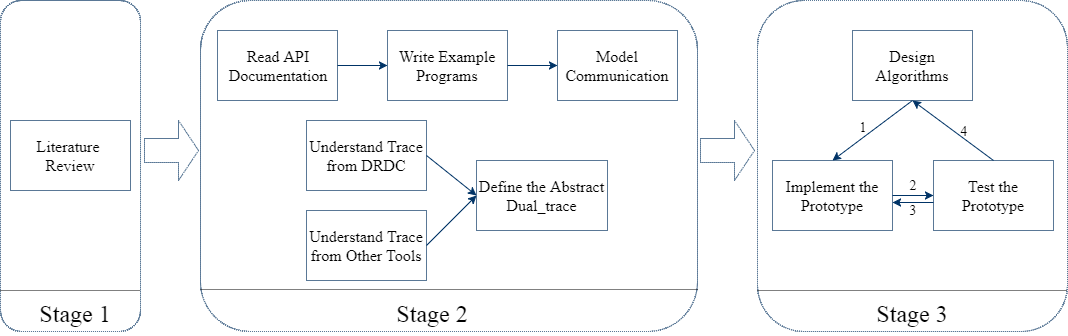
\includegraphics[scale=0.44]{Figures/methodology}}
  \caption{Research Approach overview}
  \label{methodology}
  \end{figure}

This research requires background knowledge of software security and vulnerabilities. I acquired the background knowledge basically from literature review. It helped me acquire the essential concepts of software vulnerabilities and their categories, understand some facilities for vulnerabilities detection and software maintenance in the perspective of security. After that, I was convinced that communication analysis in assembly trace level would benefit software security engineers to understand the behaviour of software and detect software vulnerabilities. 

In order to analyze the communication of programs, I had to know how the communication works. For this purpose, I started the investigation by writing simple example programs with the Windows API and run them locally in my desktop. By understanding their behaviour and reading the Windows API documentation, I abstracted the communication model which is not operating system specific.

The abstract assembly trace definition was built on the generalization of the trace format provided by our research partner, DRDC. I don't have the access to their home-made assembly tracer which is based on PIN\cite{_pin_????}. Fortunately, they provideed me with a comprehensive document about the format of the captured trace and example traces. With these, I grasped the constructive view of the assembly execution trace. Furthermore, some other tools can also capture the required information in assembly level for communication analysis. This supports the generalization of the trace definition and the abstraction of the dual\_trace.

The implementation of the prototype and the communication analysis algorithms were developed in parallel. The high level communication identification algorithm and the specific algorithms for named pipe communication method were abstracted based on the implementation, while the others are developed theoretically. Two experiments are designed to test this analysis method, the prototype and some algorithms. 


\section{Contributions}
The main contributions of this work can be summarized as:
\begin{itemize}
  \item \textbf{Communication Model:} A communication model is abstracted from the understanding of several communication methods and is generic to other communication methods. This model indicates how the communication happen in terms of what information of it has been recorded. It can guide the software analyst to analyze the communication. The analyst might be able to retrieve some information of a communication from the traces, such as a sent function call in a trace with matched received function call from the other, or the transmitted messages. However, they might not aware that they can reconstruct the communication with all the essential information as a whole picture.
  
  \item \textbf{Dual\_trace and Function Descriptor Formalization:} 
  
By understanding the assembly level execution traces, a dual\_trace was formalized to describe the information that was needed for communication analysis. The dual\_trace formalization doesn't specify the format of the execution traces but defines what information is necessary to fulfil the analysis requirement. All execution traces that comply with this formalization can be used for the analysis. This formalization can be a reference for the design of assembly tracer, guiding them what information the tracer should capture to fulfil communication analysis.

The functions descriptor describes a communication method. Following the functions descriptor formalization, the user can develop a functions descriptor through understanding the mechanism of the communication method.

  \item \textbf{Communication Analysis Approach:} The overall approach to identify the communications in the dual\_trace is designed. Eight algorithms were developed for the components in this approach regarding some communication methods or communication types. 
  
  \item \textbf{Prototype:} A prototype for communication analysis through assembly execution traces is designed and implemented on Atlantis, which is an assembly execution traces analysis environment \cite{huang2017atlantis}. Atlantis has many features that benefit the communication analysis such as view synchronization and function inspection. Moreover, the unique memory state reconstruction feature makes the data verification of a communication much easier. After the user understand the communication model and the formalization presented in this thesis, the user can use the old Atlantis (without the implementation of this prototype) to perform the analysis. However, manually identifying the communication from two traces which might contain millions lines of instructions could be an extremely time consuming and exhausting task. This prototype makes the analysis much more efficient and practical. This prototype also demonstrates that the communication analysis approach is feasible. It is a unique tool for the security engineers to analyze the communications of programs via assembly execution trace analysis. 
\end{itemize}

\section{Thesis Organization}
In Chapter 2, I summarize the related background information and knowledge needed to understand or related to this work including security and vulnerability, program communication mechanisms, program execution trace tools, and Atlantis. 

Chapter 3 describes the model of the communication between two programs. This model defines the communication in the context of trace analysis and discusses the properties of the communications. 

In Chapter 4, I first present the abstract dual\_trace formulation. Based on this formulation, I describe the communication analysis process and the essential algorithms.

In Chapter 5, I present the implementation of a dual\_trace communication analysis prototype. 

In Chapter 6, I present two experiments of communication analysis with dual\_traces using the implemented prototype. Notably, the results show the communications are correctly identified. 

Finally, in Chapter 7, I conclude the result of this research and outline possible future works.